\chapter{SYSTEM DESIGN}
This chapter details the system design of Route Optimizer, including use case models, activity diagrams, sequence diagrams, data flow diagrams, database schema design, and the user interface design philosophy.

\section{Use Case Model}
The following Use Case diagram illustrates the primary interactions between the two actors (Registered User and Anonymous Guest) and the Route Optimizer system.

\begin{figure}[H]
    \centering
    \begin{tikzpicture}[node distance=2cm, font=\small]
        % Actor - Registered User
        \node[draw, circle, minimum size=0.8cm] (user) at (-5, -1) {};
        \draw (user.south) -- (-5, -2.5);
        \draw (-5.5, -1.5) -- (-4.5, -1.5);
        \draw (-5, -2.5) -- (-5.5, -3);
        \draw (-5, -2.5) -- (-4.5, -3);
        \node[below] at (-5, -3.2) {Registered User};

        % Actor - Guest
        \node[draw, circle, minimum size=0.8cm] (guest) at (-5, -6) {};
        \draw (guest.south) -- (-5, -7.5);
        \draw (-5.5, -6.5) -- (-4.5, -6.5);
        \draw (-5, -7.5) -- (-5.5, -8);
        \draw (-5, -7.5) -- (-4.5, -8);
        \node[below] at (-5, -8.2) {Guest};

        % System Boundary
        \draw[thick] (-2.5, 1) rectangle (5, -9);
        \node at (1.25, 0.7) {\textbf{Route Optimizer System}};

        % Use Cases
        \node[draw, ellipse, minimum width=3.5cm, font=\footnotesize] (uc1) at (1.25, 0) {Register Account};
        \node[draw, ellipse, minimum width=3.5cm, font=\footnotesize] (uc2) at (1.25, -1.2) {Login};
        \node[draw, ellipse, minimum width=3.5cm, font=\footnotesize] (uc3) at (1.25, -2.4) {Search Destinations};
        \node[draw, ellipse, minimum width=3.5cm, font=\footnotesize] (uc4) at (1.25, -3.6) {Add/Remove Stops};
        \node[draw, ellipse, minimum width=3.5cm, font=\footnotesize] (uc5) at (1.25, -4.8) {Optimize Route};
        \node[draw, ellipse, minimum width=3.5cm, font=\footnotesize] (uc6) at (1.25, -6.0) {View Weather/Places};
        \node[draw, ellipse, minimum width=3.5cm, font=\footnotesize] (uc7) at (1.25, -7.2) {Save/Load/Delete Route};
        \node[draw, ellipse, minimum width=3.5cm, font=\footnotesize] (uc8) at (1.25, -8.4) {Estimate Fuel Cost};

        % Registered User Connections
        \draw (user.east) -- (uc1.west);
        \draw (user.east) -- (uc2.west);
        \draw (user.east) -- (uc3.west);
        \draw (user.east) -- (uc4.west);
        \draw (user.east) -- (uc5.west);
        \draw (user.east) -- (uc6.west);
        \draw (user.east) -- (uc7.west);
        \draw (user.east) -- (uc8.west);

        % Guest Connections
        \draw (guest.east) -- (uc1.west);
        \draw (guest.east) -- (uc2.west);
    \end{tikzpicture}
    \caption{Use Case Diagram for Route Optimizer}
    \label{fig:Use_case}
\end{figure}

\subsection{Use Case Descriptions}
\begin{table}[H]
    \centering
    \renewcommand{\arraystretch}{1.3}
    \small
    \begin{tabular}{|p{3cm}|p{3cm}|p{7cm}|}
        \hline
        \textbf{Use Case} & \textbf{Actor} & \textbf{Description} \\
        \hline
        Register Account & Guest, User & Create a new user account with name, email, and password \\
        \hline
        Login & Guest, User & Authenticate using email and password to receive a JWT \\
        \hline
        Search Destinations & Registered User & Search for a location via Photon geocoding autocomplete \\
        \hline
        Add/Remove Stops & Registered User & Build the trip itinerary by adding or removing destination stops \\
        \hline
        Optimize Route & Registered User & Run the Nearest Neighbor algorithm to reorder stops efficiently \\
        \hline
        View Weather/Places & Registered User & View real-time weather, nearby hotels, and fuel stations for each stop \\
        \hline
        Save/Load/Delete Route & Registered User & Persist, retrieve, or remove itineraries from the cloud database \\
        \hline
        Estimate Fuel Cost & Registered User & Calculate trip fuel cost based on mileage and fuel price inputs \\
        \hline
    \end{tabular}
    \caption{Use Case Descriptions}
    \label{tab:use_case_desc}
\end{table}

\section{Activity Diagrams}

\subsection{User Authentication Flow}
\begin{figure}[H]
    \centering
    \begin{tikzpicture}[node distance=1.5cm, auto, >=stealth]
        \node[draw, circle, fill=black, inner sep=2pt] (start) {};
        \node[draw, rounded corners, below of=start] (input) {Enter Email \& Password};
        \node[draw, diamond, aspect=2, below of=input, node distance=2cm] (check) {Valid?};
        \node[draw, rounded corners, below of=check, node distance=2cm] (auth) {Generate JWT Token};
        \node[draw, rounded corners, left of=check, node distance=4cm] (fail) {Display Error Message};
        \node[draw, rounded corners, below of=auth] (store) {Store Token in LocalStorage};
        \node[draw, rounded corners, below of=store] (redirect) {Redirect to Dashboard};
        \node[draw, double, circle, below of=redirect, inner sep=2pt] (end) {};

        \path[draw, ->] (start) -- (input);
        \path[draw, ->] (input) -- (check);
        \path[draw, ->] (check) -- node {Yes} (auth);
        \path[draw, ->] (check) -- node {No} (fail);
        \path[draw, ->] (fail) |- (input);
        \path[draw, ->] (auth) -- (store);
        \path[draw, ->] (store) -- (redirect);
        \path[draw, ->] (redirect) -- (end);
    \end{tikzpicture}
    \caption{Activity Diagram -- User Authentication Flow}
    \label{fig:Auth_activity}
\end{figure}

\subsection{Complete Itinerary Planning Flow}
\begin{figure}[H]
    \centering
    \begin{tikzpicture}[node distance=1.3cm, auto, >=stealth, font=\footnotesize]
        \node[draw, circle, fill=black, inner sep=2pt] (start) {};
        \node[draw, rounded corners, below of=start] (search) {Search Location (Photon API)};
        \node[draw, rounded corners, below of=search] (select) {Select from Autocomplete Results};
        \node[draw, rounded corners, below of=select] (add) {Add Stop to Itinerary};
        \node[draw, diamond, aspect=2.5, below of=add, node distance=1.8cm] (more) {More stops?};
        \node[draw, rounded corners, below of=more, node distance=1.8cm] (optimize) {Trigger Route Optimization};
        \node[draw, rounded corners, below of=optimize] (haversine) {Calculate Haversine Distances};
        \node[draw, rounded corners, below of=haversine] (nn) {Apply Nearest Neighbor Algorithm};
        \node[draw, rounded corners, below of=nn] (enrich) {Fetch Weather \& Nearby Places};
        \node[draw, rounded corners, below of=enrich] (display) {Display Optimized Itinerary};
        \node[draw, diamond, aspect=2.5, below of=display, node distance=1.8cm] (save) {Save trip?};
        \node[draw, rounded corners, below of=save, node distance=1.8cm] (persist) {POST to /api/routes (with JWT)};
        \node[draw, double, circle, below of=persist, inner sep=2pt] (end) {};

        \path[draw, ->] (start) -- (search);
        \path[draw, ->] (search) -- (select);
        \path[draw, ->] (select) -- (add);
        \path[draw, ->] (add) -- (more);
        \path[draw, ->] (more) -- node {No} (optimize);
        \path[draw, ->] (more.east) -- ++(2,0) |- node[near start, right] {Yes} (search.east);
        \path[draw, ->] (optimize) -- (haversine);
        \path[draw, ->] (haversine) -- (nn);
        \path[draw, ->] (nn) -- (enrich);
        \path[draw, ->] (enrich) -- (display);
        \path[draw, ->] (display) -- (save);
        \path[draw, ->] (save) -- node {Yes} (persist);
        \path[draw, ->] (save.east) -- ++(1.5,0) |- (end.east);
        \path[draw, ->] (persist) -- (end);
    \end{tikzpicture}
    \caption{Activity Diagram -- Complete Itinerary Planning Flow}
    \label{fig:Full_activity}
\end{figure}

\subsection{Route Save and Load Flow}
\begin{figure}[H]
    \centering
    \begin{tikzpicture}[node distance=1.5cm, auto, >=stealth, font=\footnotesize]
        \node[draw, circle, fill=black, inner sep=2pt] (start) {};
        \node[draw, rounded corners, below of=start] (open) {Open Trip Dashboard};
        \node[draw, rounded corners, below of=open] (fetch) {GET /api/routes (with JWT)};
        \node[draw, rounded corners, below of=fetch] (display) {Display Saved Route Cards};
        \node[draw, diamond, aspect=2, below of=display, node distance=2cm] (action) {Action?};
        \node[draw, rounded corners, right of=action, node distance=4cm] (load) {Load Route Details};
        \node[draw, rounded corners, left of=action, node distance=4cm] (delete) {DELETE /api/routes/:id};
        \node[draw, rounded corners, below of=load] (view) {Display Full Itinerary};
        \node[draw, rounded corners, below of=delete] (confirm) {Remove from List};
        \node[draw, double, circle, below of=action, node distance=4cm] (end) {};

        \path[draw, ->] (start) -- (open);
        \path[draw, ->] (open) -- (fetch);
        \path[draw, ->] (fetch) -- (display);
        \path[draw, ->] (display) -- (action);
        \path[draw, ->] (action) -- node {Load} (load);
        \path[draw, ->] (action) -- node {Delete} (delete);
        \path[draw, ->] (load) -- (view);
        \path[draw, ->] (delete) -- (confirm);
        \path[draw, ->] (view) |- (end);
        \path[draw, ->] (confirm) |- (end);
    \end{tikzpicture}
    \caption{Activity Diagram -- Route Save and Load Flow}
    \label{fig:SaveLoad_activity}
\end{figure}

\section{Sequence Diagrams}

\subsection{User Registration Sequence}
\begin{figure}[H]
    \centering
    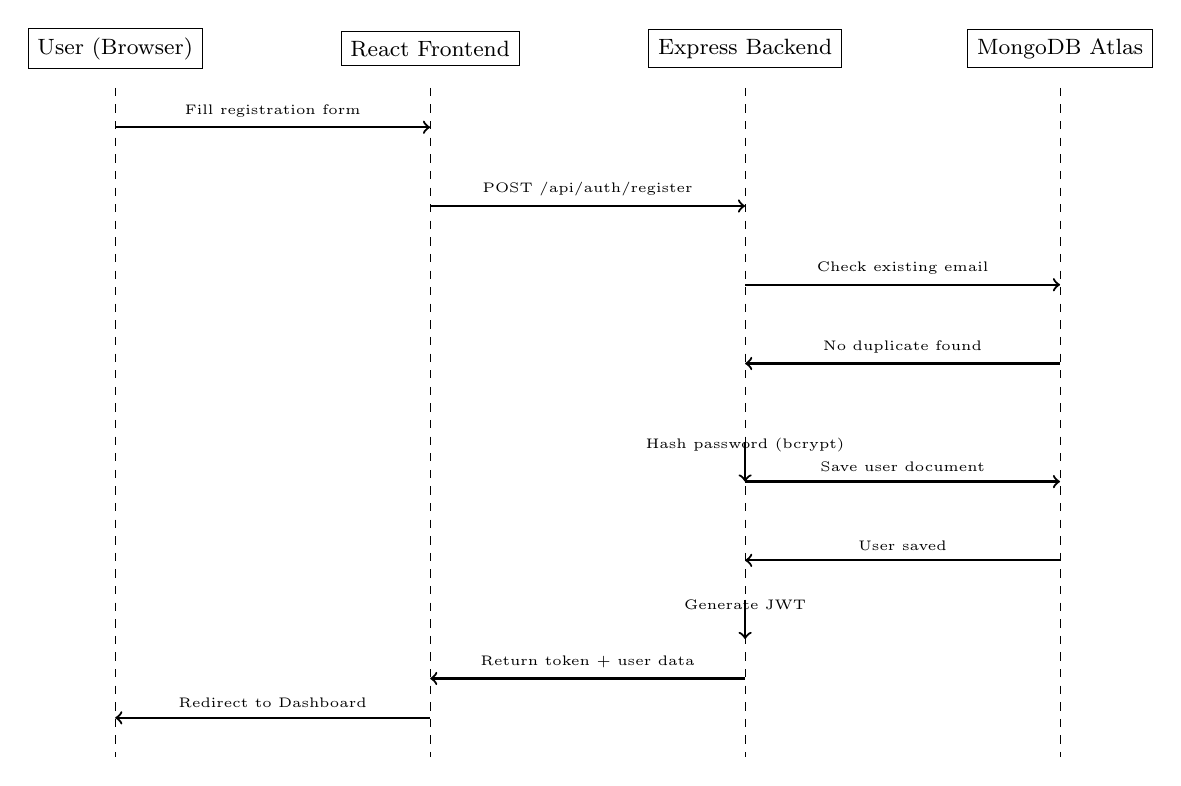
\begin{tikzpicture}[font=\footnotesize]
        % Lifelines
        \node[draw, rectangle] (user) at (0, 0) {User (Browser)};
        \node[draw, rectangle] (fe) at (4, 0) {React Frontend};
        \node[draw, rectangle] (be) at (8, 0) {Express Backend};
        \node[draw, rectangle] (db) at (12, 0) {MongoDB Atlas};

        \draw[dashed] (0, -0.5) -- (0, -9);
        \draw[dashed] (4, -0.5) -- (4, -9);
        \draw[dashed] (8, -0.5) -- (8, -9);
        \draw[dashed] (12, -0.5) -- (12, -9);

        % Messages
        \draw[->, thick] (0, -1) -- node[above, font=\tiny] {Fill registration form} (4, -1);
        \draw[->, thick] (4, -2) -- node[above, font=\tiny] {POST /api/auth/register} (8, -2);
        \draw[->, thick] (8, -3) -- node[above, font=\tiny] {Check existing email} (12, -3);
        \draw[<-, thick] (8, -4) -- node[above, font=\tiny] {No duplicate found} (12, -4);
        \draw[->, thick] (8, -5) -- node[above, font=\tiny] {Hash password (bcrypt)} (8, -5.5);
        \draw[->, thick] (8, -5.5) -- node[above, font=\tiny] {Save user document} (12, -5.5);
        \draw[<-, thick] (8, -6.5) -- node[above, font=\tiny] {User saved} (12, -6.5);
        \draw[->, thick] (8, -7) -- node[above, font=\tiny] {Generate JWT} (8, -7.5);
        \draw[<-, thick] (4, -8) -- node[above, font=\tiny] {Return token + user data} (8, -8);
        \draw[<-, thick] (0, -8.5) -- node[above, font=\tiny] {Redirect to Dashboard} (4, -8.5);
    \end{tikzpicture}
    \caption{Sequence Diagram -- User Registration}
    \label{fig:Reg_sequence}
\end{figure}

\subsection{Route Optimization Sequence}
\begin{figure}[H]
    \centering
    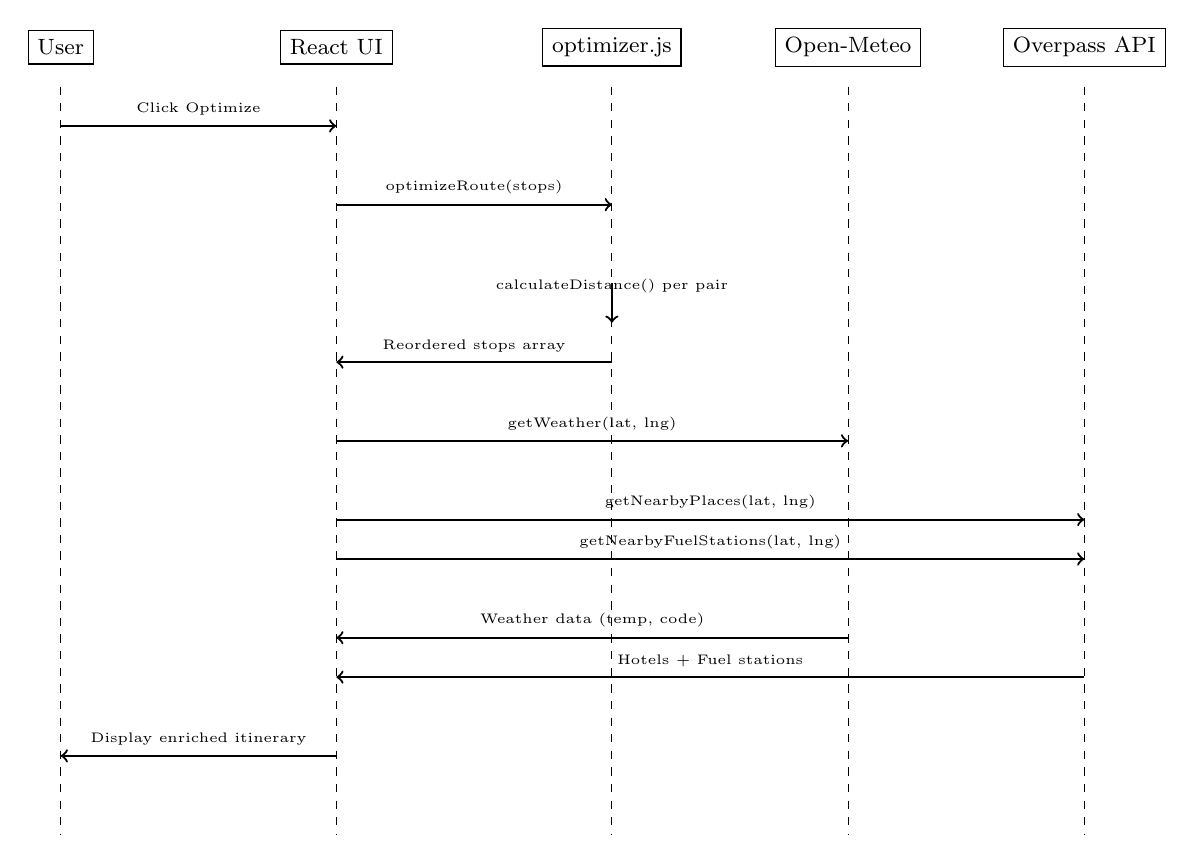
\begin{tikzpicture}[font=\footnotesize]
        % Lifelines
        \node[draw, rectangle] (user) at (0, 0) {User};
        \node[draw, rectangle] (fe) at (3.5, 0) {React UI};
        \node[draw, rectangle] (opt) at (7, 0) {optimizer.js};
        \node[draw, rectangle] (wea) at (10, 0) {Open-Meteo};
        \node[draw, rectangle] (osm) at (13, 0) {Overpass API};

        \draw[dashed] (0, -0.5) -- (0, -10);
        \draw[dashed] (3.5, -0.5) -- (3.5, -10);
        \draw[dashed] (7, -0.5) -- (7, -10);
        \draw[dashed] (10, -0.5) -- (10, -10);
        \draw[dashed] (13, -0.5) -- (13, -10);

        \draw[->, thick] (0, -1) -- node[above, font=\tiny] {Click Optimize} (3.5, -1);
        \draw[->, thick] (3.5, -2) -- node[above, font=\tiny] {optimizeRoute(stops)} (7, -2);
        \draw[->, thick] (7, -3) -- node[above, font=\tiny] {calculateDistance() per pair} (7, -3.5);
        \draw[<-, thick] (3.5, -4) -- node[above, font=\tiny] {Reordered stops array} (7, -4);
        \draw[->, thick] (3.5, -5) -- node[above, font=\tiny] {getWeather(lat, lng)} (10, -5);
        \draw[->, thick] (3.5, -6) -- node[above, font=\tiny] {getNearbyPlaces(lat, lng)} (13, -6);
        \draw[->, thick] (3.5, -6.5) -- node[above, font=\tiny] {getNearbyFuelStations(lat, lng)} (13, -6.5);
        \draw[<-, thick] (3.5, -7.5) -- node[above, font=\tiny] {Weather data (temp, code)} (10, -7.5);
        \draw[<-, thick] (3.5, -8) -- node[above, font=\tiny] {Hotels + Fuel stations} (13, -8);
        \draw[<-, thick] (0, -9) -- node[above, font=\tiny] {Display enriched itinerary} (3.5, -9);
    \end{tikzpicture}
    \caption{Sequence Diagram -- Route Optimization and Data Enrichment}
    \label{fig:Opt_sequence}
\end{figure}

\subsection{Admin Dashboard Sequence}
\begin{figure}[H]
    \centering
    \begin{tikzpicture}[font=\footnotesize]
        % Lifelines
        \node[draw, rectangle] (admin) at (0, 0) {Admin User};
        \node[draw, rectangle] (fe) at (4, 0) {React Frontend};
        \node[draw, rectangle] (be) at (8, 0) {Express Backend};
        \node[draw, rectangle] (db) at (12, 0) {MongoDB Atlas};

        \draw[dashed] (0, -0.5) -- (0, -8);
        \draw[dashed] (4, -0.5) -- (4, -8);
        \draw[dashed] (8, -0.5) -- (8, -8);
        \draw[dashed] (12, -0.5) -- (12, -8);

        % Messages
        \draw[->, thick] (0, -1) -- node[above, font=\tiny] {Navigates to /admin/dashboard} (4, -1);
        \draw[->, thick] (4, -2) -- node[above, font=\tiny] {GET /api/admin/users \& /routes (with JWT)} (8, -2);
        \draw[->, thick] (8, -3) -- node[above, font=\tiny] {Verify adminAuth Middleware} (8, -3.5);
        \draw[->, thick] (8, -4) -- node[above, font=\tiny] {Query all users \& routes} (12, -4);
        \draw[<-, thick] (8, -5) -- node[above, font=\tiny] {Return aggregated documents} (12, -5);
        \draw[<-, thick] (4, -6) -- node[above, font=\tiny] {Return JSON arrays} (8, -6);
        \draw[<-, thick] (0, -7) -- node[above, font=\tiny] {Render Admin Tables & Stats} (4, -7);
    \end{tikzpicture}
    \caption{Sequence Diagram -- Admin Dashboard Data Flow}
    \label{fig:Admin_sequence}
\end{figure}

\section{Database Schema Design}
The Route Optimizer backend uses MongoDB with Mongoose ODM for data modeling. Two primary collections are used:

\subsection{User Collection Schema}
\begin{lstlisting}[style=csharpstyle]
const userSchema = new mongoose.Schema({
    name: {
        type: String,
        required: true,
        trim: true
    },
    email: {
        type: String,
        required: true,
        unique: true,
        lowercase: true,
        trim: true
    },
    password: {
        type: String,
        required: true,
        minlength: 6
    }
}, { timestamps: true });

// Pre-save hook: hash password with bcrypt (10 salt rounds)
// Instance method: comparePassword() for login verification
\end{lstlisting}

The \texttt{timestamps: true} option automatically adds \texttt{createdAt} and \texttt{updatedAt} fields to every document, providing audit trail capabilities.

\subsection{Route Collection Schema}
\begin{lstlisting}[style=csharpstyle]
const routeSchema = new mongoose.Schema({
    userId: {
        type: mongoose.Schema.Types.ObjectId,
        ref: 'User',
        required: true
    },
    name: { type: String, required: true, trim: true },
    date: { type: String, required: true },
    totalDistance: { type: Number, default: 0 },
    totalStops: { type: Number, default: 0 },
    estimatedCost: { type: Number, default: 0 },
    estimatedTime: { type: Number, default: 0 },
    stops: { type: Array, default: [] },
    metrics: { type: Object, default: {} }
}, { timestamps: true });
\end{lstlisting}

The \texttt{userId} field establishes a reference relationship to the User collection, enabling data isolation. The top-level summary fields (\texttt{totalDistance}, \texttt{totalStops}, etc.) are denormalized for efficient listing in the dashboard without needing to parse the nested \texttt{stops} array.

\subsection{Sample Route Document}
\begin{lstlisting}[style=csharpstyle]
{
    "_id": "ObjectId(...)  ",
    "userId": "ObjectId(...)",
    "name": "Summer Road Trip",
    "date": "2026-06-15",
    "totalDistance": 450.5,
    "totalStops": 5,
    "estimatedCost": 3500,
    "estimatedTime": 540,
    "stops": [
        {
            "name": "Kochi, Kerala, India",
            "lat": 9.9312,
            "lng": 76.2673,
            "weather": { "temp": 28, "description": "Clear sky" }
        },
        {
            "name": "Munnar, Kerala, India",
            "lat": 10.0889,
            "lng": 77.0595,
            "weather": { "temp": 18, "description": "Partly cloudy" }
        }
    ],
    "metrics": {
        "totalDistance": 450.5,
        "estimatedCost": 3500,
        "estimatedTime": 540
    },
    "createdAt": "2026-06-15T10:30:00Z",
    "updatedAt": "2026-06-15T10:30:00Z"
}
\end{lstlisting}

\section{API Endpoint Design}
The backend exposes a RESTful API organized into two route groups:

\begin{table}[H]
    \centering
    \renewcommand{\arraystretch}{1.4}
    \small
    \begin{tabular}{|p{2cm}|p{3.5cm}|p{2cm}|p{5.5cm}|}
        \hline
        \textbf{Method} & \textbf{Endpoint} & \textbf{Auth} & \textbf{Description} \\
        \hline
        POST & /api/auth/register & No & Register new user, return JWT \\
        \hline
        POST & /api/auth/login & No & Authenticate user, return JWT \\
        \hline
        GET & /api/routes & Yes (JWT) & Fetch all routes for logged-in user \\
        \hline
        POST & /api/routes & Yes (JWT) & Save a new optimized route \\
        \hline
        DELETE & /api/routes/:id & Yes (JWT) & Delete a specific saved route \\
        \hline
        GET & /api/admin/users & Yes (Admin JWT) & Fetch all registered users \\
        \hline
        GET & /api/admin/routes & Yes (Admin JWT) & Fetch all created routes globally \\
        \hline
        GET & /api/health & No & Server health check \\
        \hline
    \end{tabular}
    \caption{REST API Endpoints}
    \label{tab:api_endpoints}
\end{table}

\section{Project Design}
The design of Route Optimizer focuses on providing a premium digital experience that simplifies complex geospatial data into an actionable travel plan. The application is designed to be mobile-responsive and visually engaging, utilizing a ``Glassmorphic'' design system characterized by blurred backgrounds and translucent overlays that create a sense of depth and hierarchy.\\\\
At its core, the project design balances technical utility with aesthetic excellence. The dashboard provides clear sections for tool panels (input, saved routes, settings) and specialized view switchers that allow users to toggle between a planning list, an immersive map view, and trip insights (metrics).

\subsection{UI Design}
The UI is built using React with a focus on immersive interaction. Key design elements include:
\begin{itemize}
    \item \textbf{Immersive Backgrounds:} Dynamic animated gradient ``blobs'' using CSS keyframe animations provide a high-end, living feel that distinguishes the app from static interfaces.
    \item \textbf{Glass Containers:} Functional panels use CSS \texttt{backdrop-filter: blur()} and semi-transparent backgrounds (\texttt{rgba()}) to maintain readability while subtly revealing the animated background layers through the panels.
    \item \textbf{Micro-interactions:} Buttons feature smooth \texttt{transform: scale()} transitions on hover. Cards display elevation changes and subtle shadow effects. Icons from the Lucide-React library feature jiggle animations triggered by user interaction.
    \item \textbf{Responsive Layout:} CSS media queries ensure the interface adapts gracefully from wide desktop monitors to narrow tablet or mobile screens, reflows panels vertically, and adjusts font sizes proportionally.
    \item \textbf{Consistent Design System:} Reusable \texttt{Button} and \texttt{Input} components with dedicated CSS files enforce visual consistency. Each component accepts props for variant styling (primary, secondary, danger) and size configurations.
\end{itemize}

\subsection{Application Screenshots}
The following screenshots showcase the key screens and user interface elements of the Route Optimizer application, demonstrating the glassmorphic design system and responsive layout in action.

\subsubsection{Landing Page}
The landing page serves as the entry point for new visitors, presenting the application's core value proposition with the tagline ``Plan the perfect road trip.'' It highlights three key features --- Smart Routes, Live Weather, and Curated Stays --- using vibrant icon cards. A prominent ``Get Started'' call-to-action button with a gradient finish guides users towards registration.

\begin{figure}[H]
    \centering
    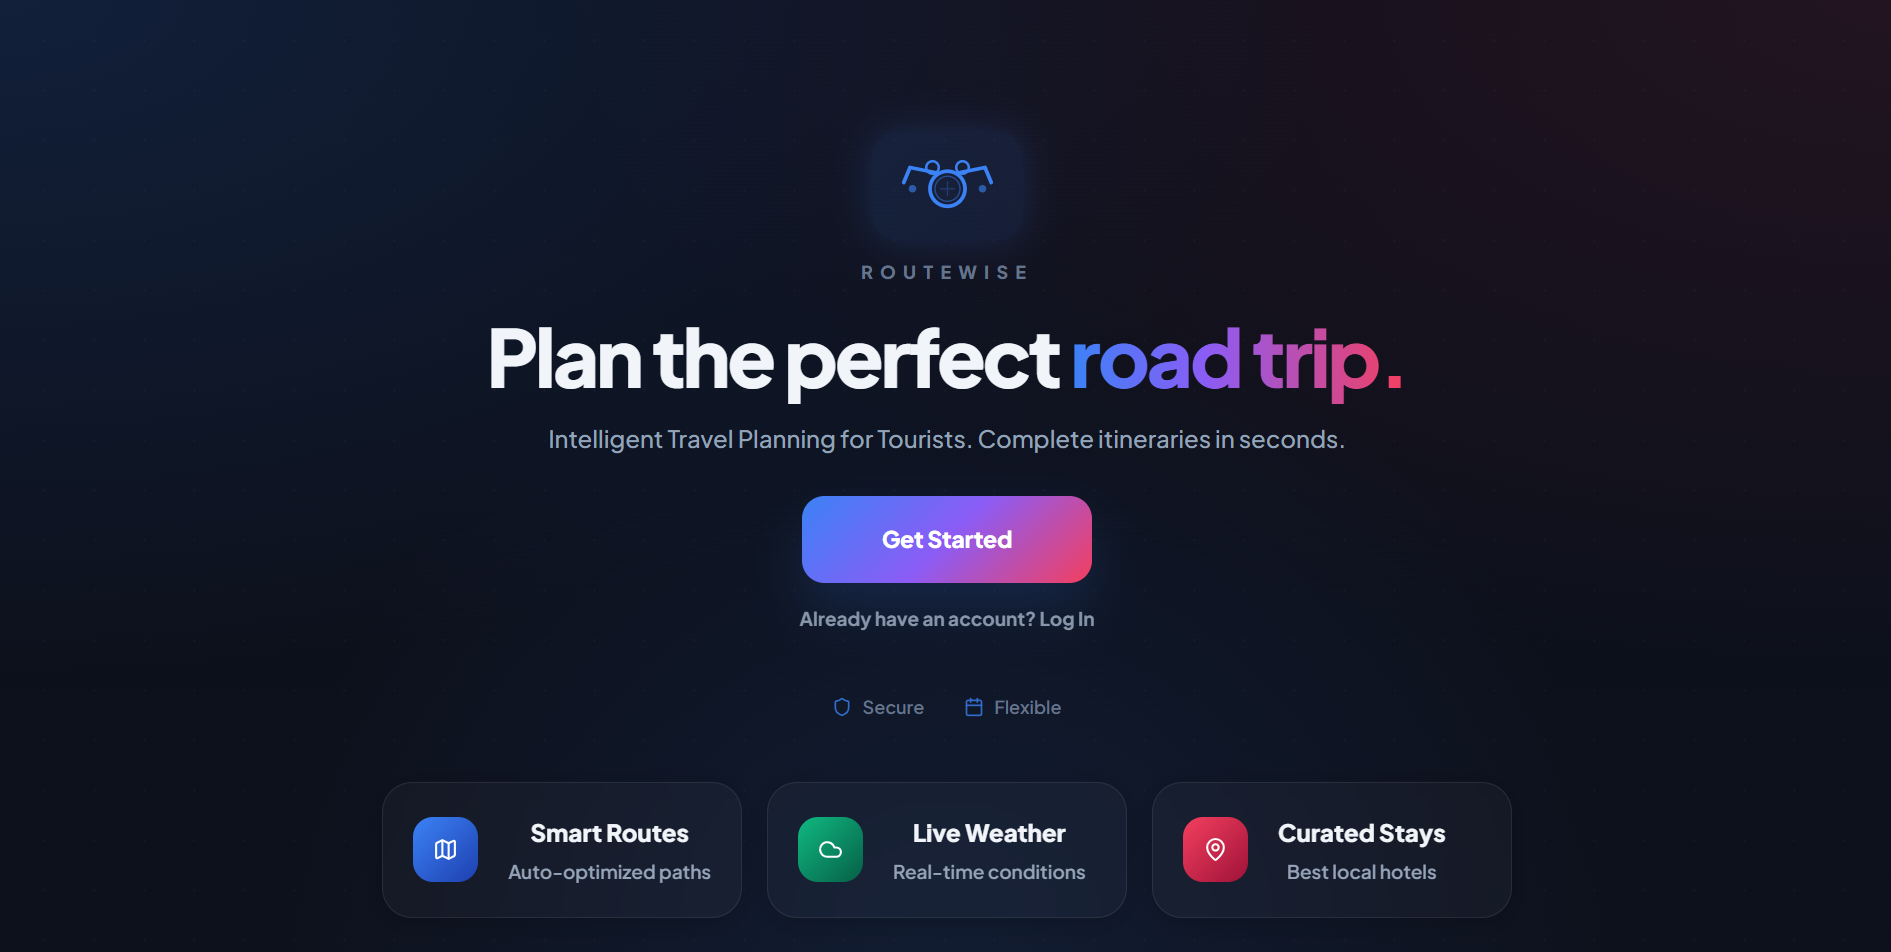
\includegraphics[width=\textwidth]{screenshots/Interface.png}
    \caption{Landing Page -- Route Optimizer Interface}
    \label{fig:ss_landing}
\end{figure}

\subsubsection{Registration Page}
The registration screen provides a clean, centered form for new user onboarding. Users are required to enter their Full Name, Email, and Password. The form is enclosed in a glassmorphic container with a translucent border, maintaining the application's dark-themed aesthetic. A link to the login page is provided for users who already have an account.

\begin{figure}[H]
    \centering
    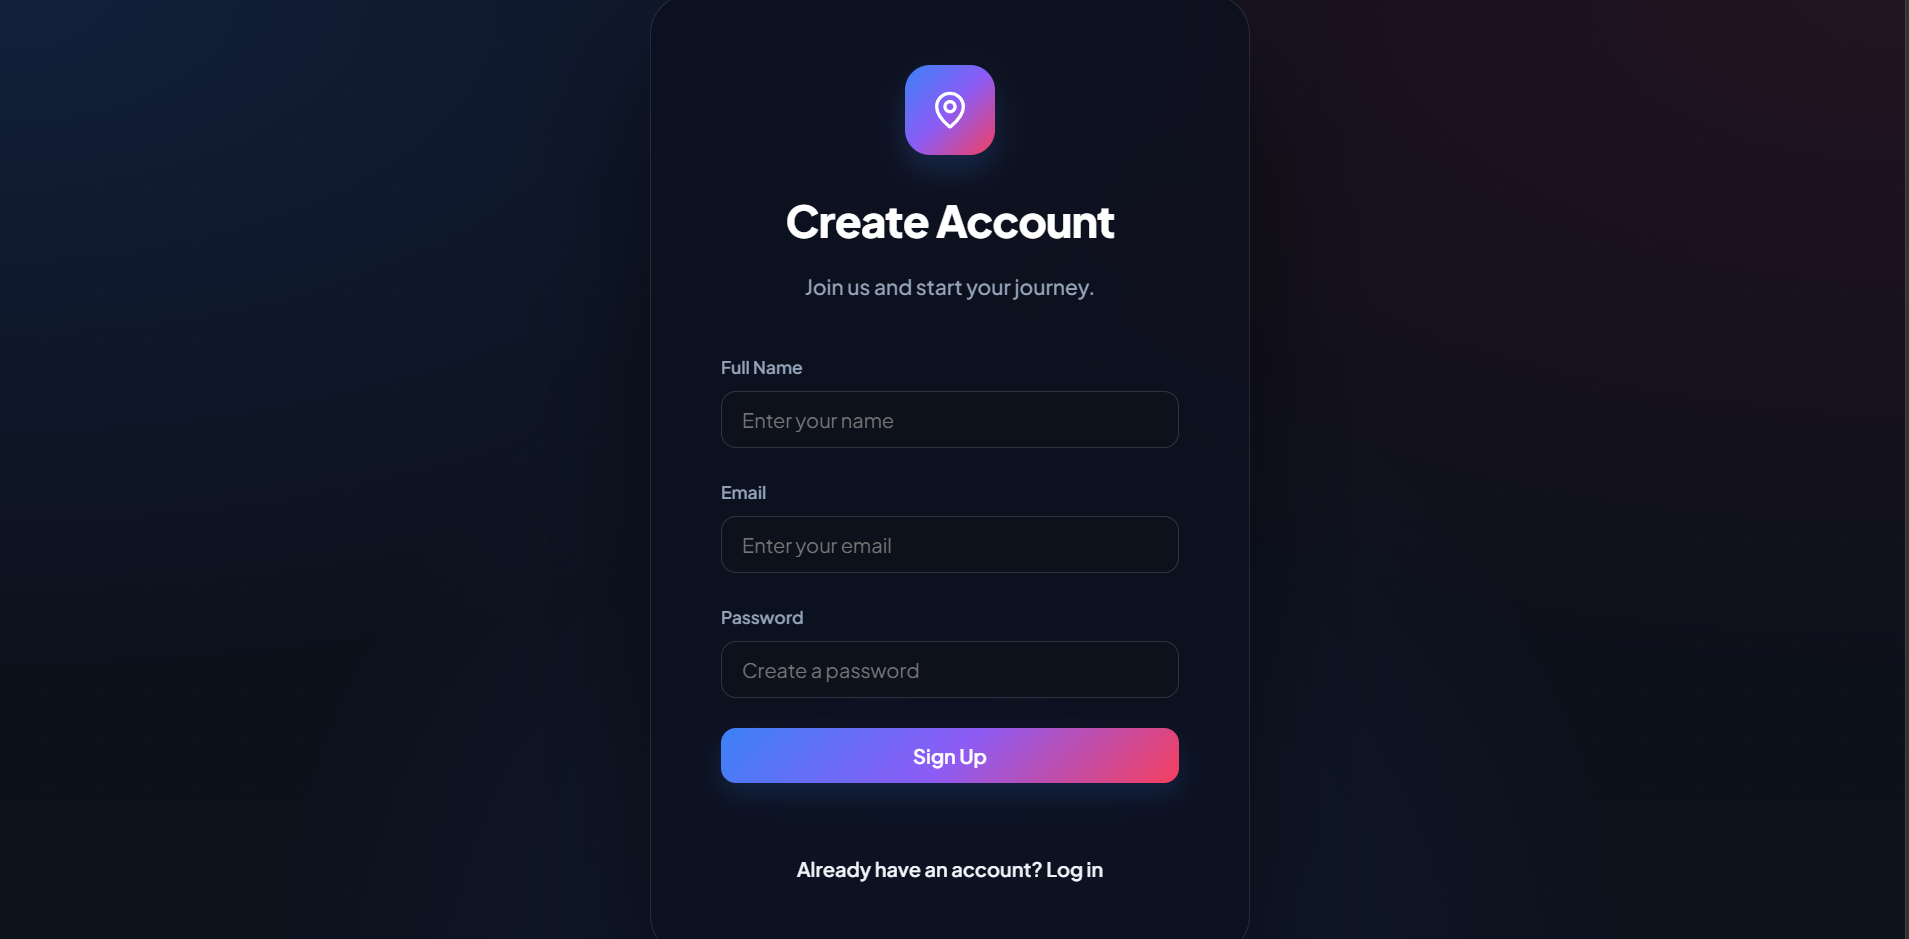
\includegraphics[width=0.85\textwidth]{screenshots/Registration page.png}
    \caption{User Registration Page}
    \label{fig:ss_register}
\end{figure}

\subsubsection{Login Page}
The login page features a minimalist design with Email and Password input fields. The ``Welcome Back'' heading and the descriptive subtitle ``Plan your perfect trip with ease'' reinforce the application's purpose. A gradient ``Log In'' button and a redirect link for new users complete the authentication interface.

\begin{figure}[H]
    \centering
    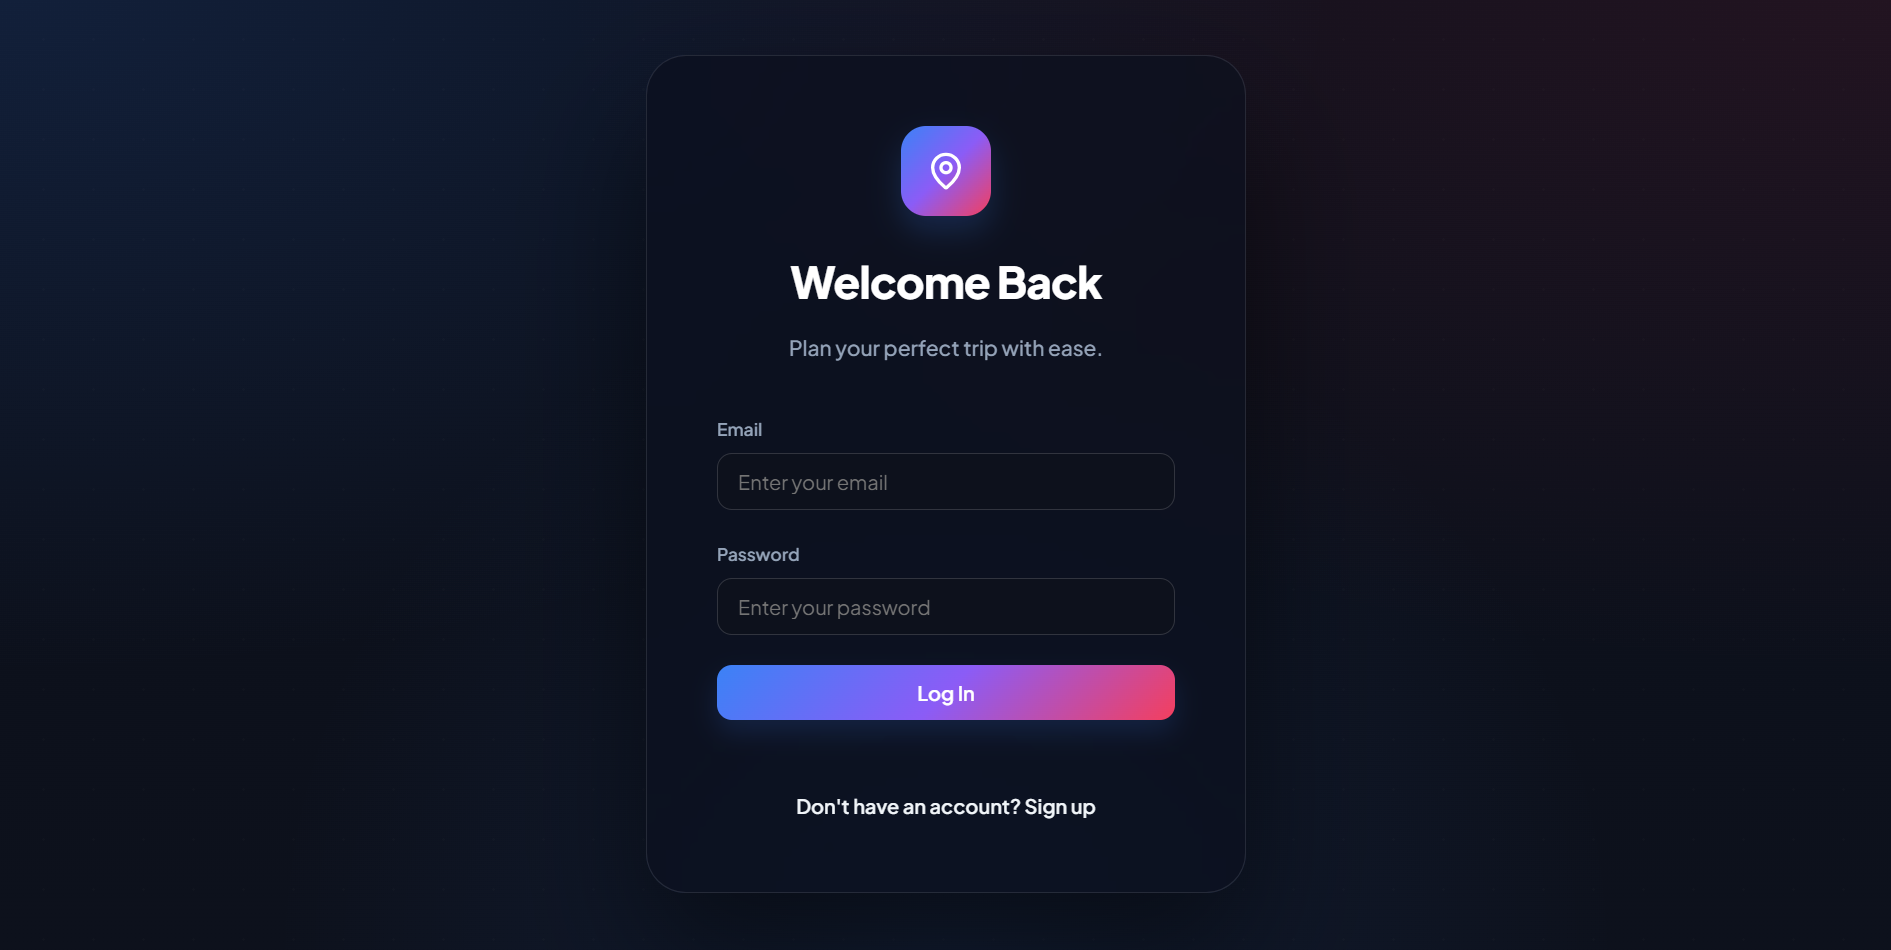
\includegraphics[width=0.85\textwidth]{screenshots/Login page.png}
    \caption{User Login Page}
    \label{fig:ss_login}
\end{figure}

\subsubsection{User Dashboard -- Planner View}
The main dashboard is presented in the ``Planner'' tab and serves as the primary workspace for trip planning. The left panel contains a destination search bar with autocomplete functionality and a Vehicle Settings section where users can configure their vehicle's mileage (km/l) and fuel price (per liter) for cost estimation. The right panel displays the current itinerary status. A tab switcher at the top allows navigation between Planner, Map, and Insights views.

\begin{figure}[H]
    \centering
    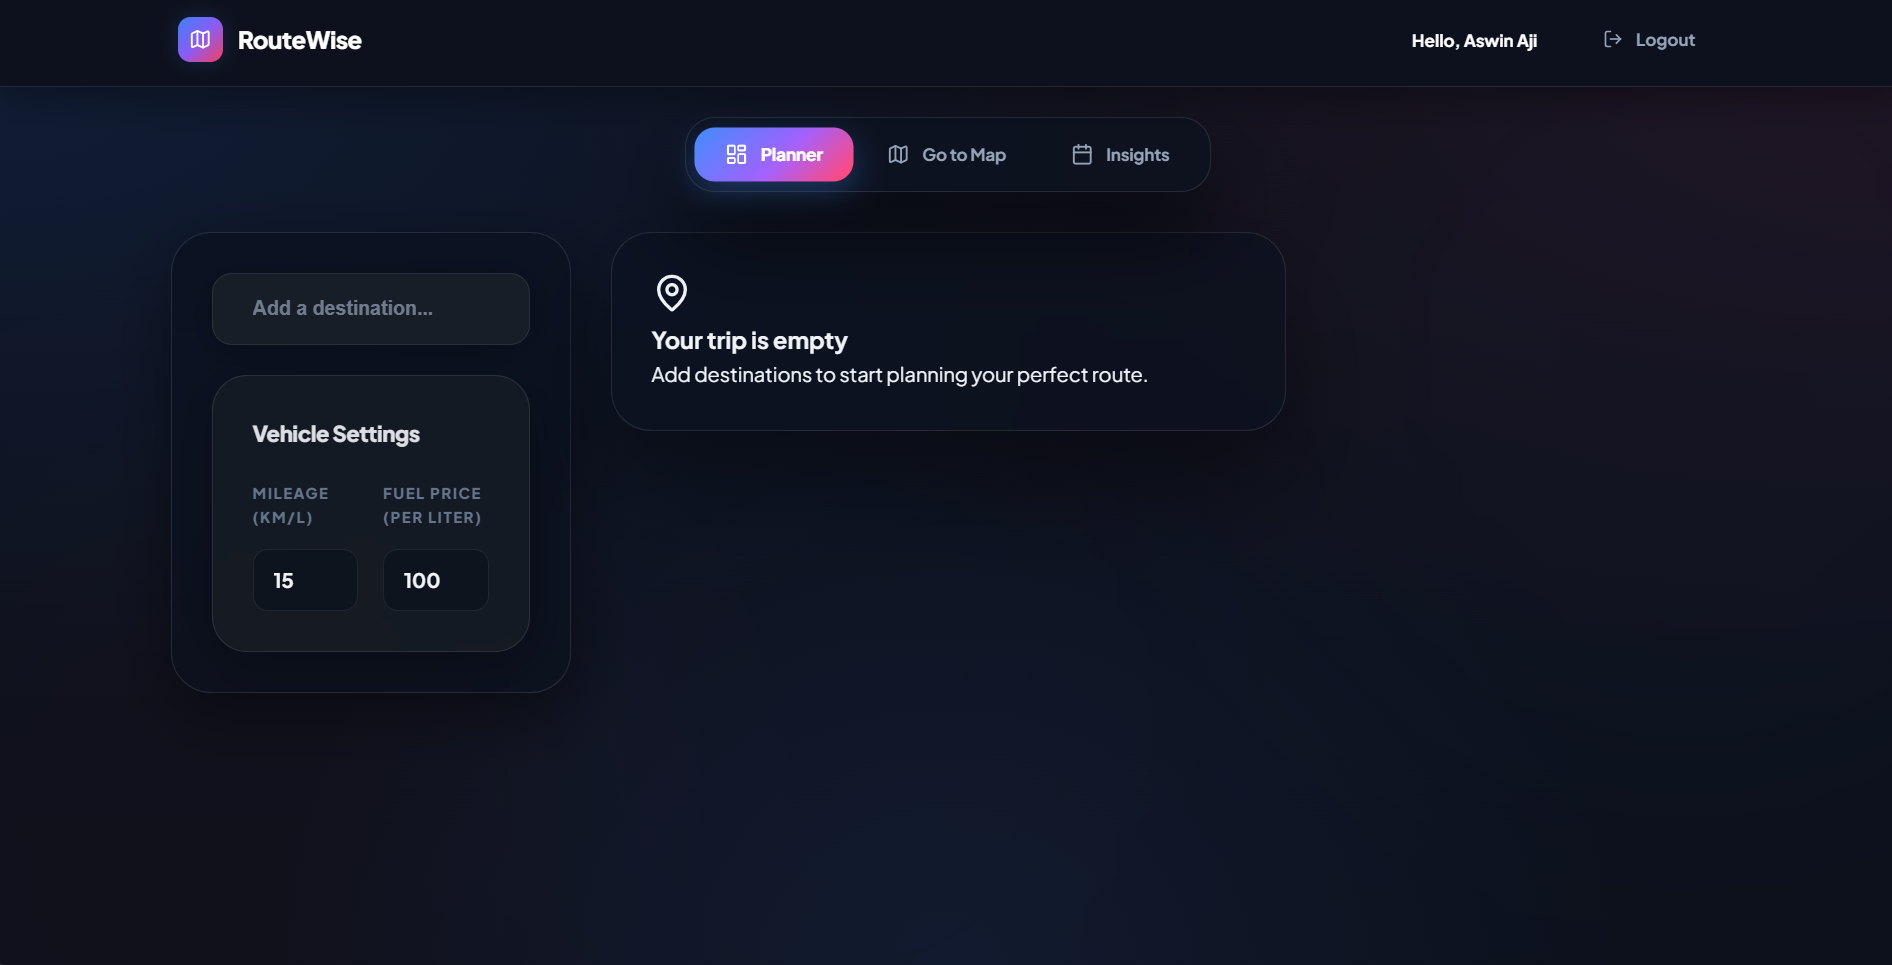
\includegraphics[width=\textwidth]{screenshots/User Dashboard.png}
    \caption{User Dashboard -- Planner View}
    \label{fig:ss_dashboard}
\end{figure}

\subsubsection{Map View}
The ``Go to Map'' tab renders a full-screen interactive map powered by Leaflet.js with OpenStreetMap tile layers. This view allows users to visualize their planned route geographically, with markers placed at each destination stop. The map supports zoom controls and panning, providing a spatial overview of the entire trip itinerary.

\begin{figure}[H]
    \centering
    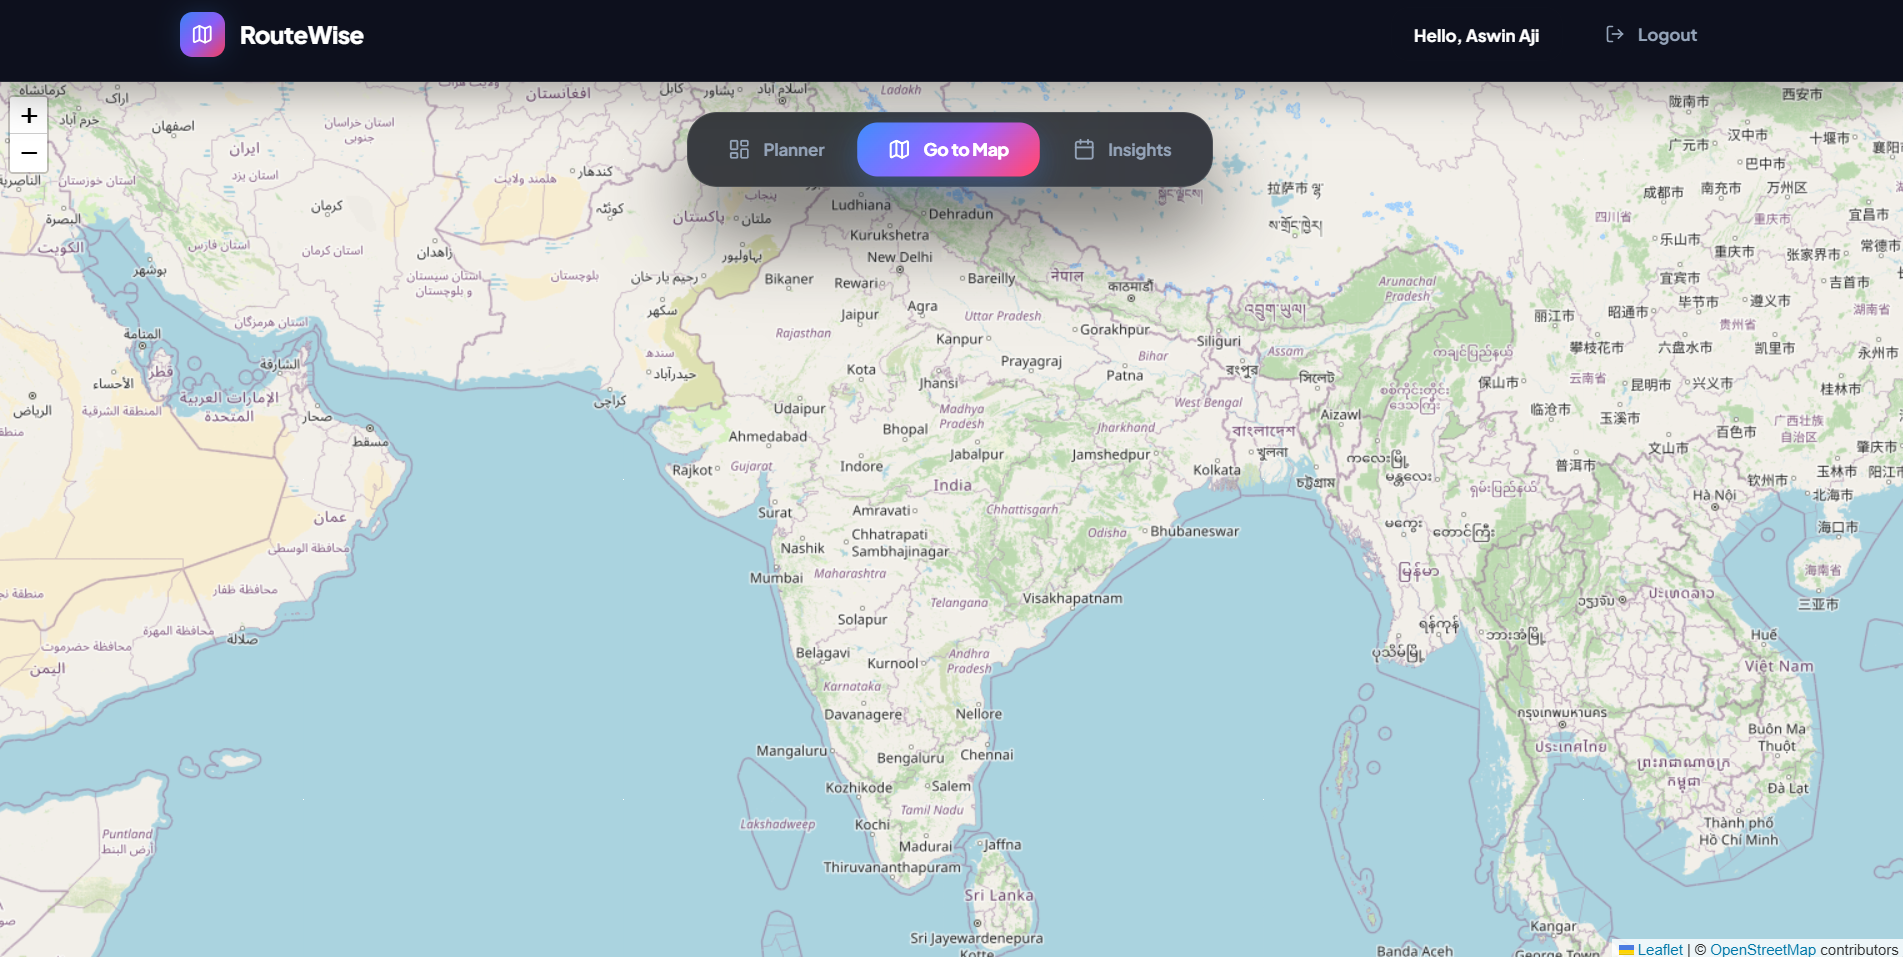
\includegraphics[width=\textwidth]{screenshots/Map.png}
    \caption{Interactive Map View with Leaflet and OpenStreetMap}
    \label{fig:ss_map}
\end{figure}

\subsubsection{Insights Panel}
The ``Insights'' tab provides a high-level summary of the user's travel history. It displays three key metrics in glassmorphic stat cards: Trips Completed, Total Distance (in km), and Fuel Investment (in INR). This panel aggregates data from all saved routes to give users a quick overview of their travel activity and expenditure over time.

\begin{figure}[H]
    \centering
    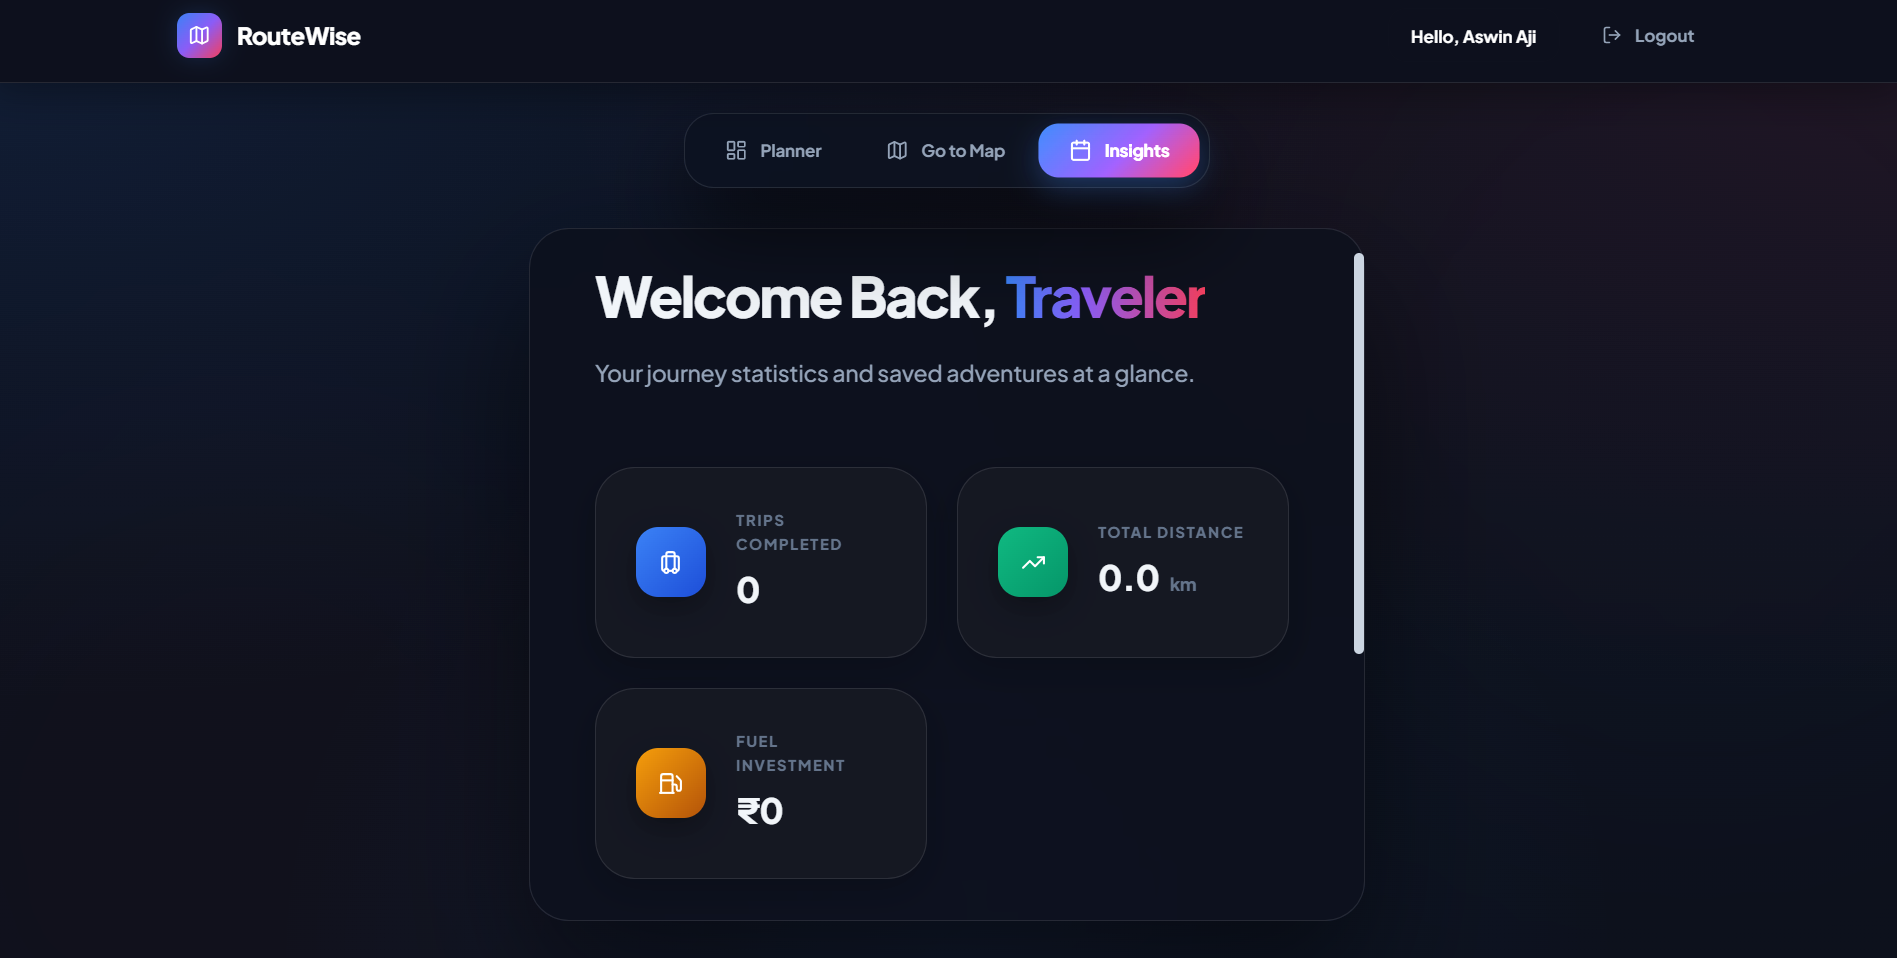
\includegraphics[width=\textwidth]{screenshots/Insights.png}
    \caption{Trip Insights and Statistics Panel}
    \label{fig:ss_insights}
\end{figure}

\subsubsection{Admin Dashboard}
The Admin Dashboard is an exclusive, secure interface accessible only to users with the Administrator role. It provides platform-wide oversight, featuring high-level statistics cards (Total Users, Total Routes) and two detailed data tables. The User Management table displays all registered accounts with their respective roles, while the Route Analytics table grants visibility into every itinerary created on the platform, fostering better administrative control.

\begin{figure}[H]
    \centering
    \includegraphics[width=\textwidth]{screenshots/Admin Dashboard.png} % Replace with actual screenshot path when added
    \caption{Admin Dashboard -- User Management View}
    \label{fig:ss_admin_dashboard}
\end{figure}

\subsection{Component Architecture}
The frontend follows a modular component hierarchy:
\begin{itemize}
    \item \textbf{App.jsx:} Root component managing routes (Login, Register, Home pages).
    \item \textbf{Pages:} \texttt{Home.jsx} (main dashboard, 580+ lines), \texttt{Login.jsx}, \texttt{Register.jsx}.
    \item \textbf{Dashboard Components:}
    \begin{itemize}
        \item \texttt{SpotForm.jsx} -- Location search with autocomplete
        \item \texttt{SpotList.jsx} -- Added stops management
        \item \texttt{RouteResult.jsx} -- Optimized itinerary display with weather, hotels, fuel
        \item \texttt{MapPreview.jsx} -- Interactive map visualization
        \item \texttt{FuelSettings.jsx} -- Vehicle mileage and fuel price input
        \item \texttt{SavedRoutes.jsx} -- Saved trip card list
        \item \texttt{TripDashboard.jsx} -- Full trip history management
    \end{itemize}
    \item \textbf{Common:} \texttt{Button.jsx/css}, \texttt{Input.jsx/css} -- Reusable styled primitives.
    \item \textbf{Context:} \texttt{AuthContext} -- Global authentication state provider.
    \item \textbf{Utils:} \texttt{geocoding.js}, \texttt{optimizer.js}, \texttt{weather.js}, \texttt{places.js}.
\end{itemize}
